\section{Einleitung}\raggedbottom 

In dieser Bachelorarbeit wird untersucht inwieweit Lineare Programmierung als Hilfsmittel für eine Contig-Assemblierung eingesetzt werden kann, anhand von Contigs aus der MHC (Haupthistokompatibilitätskomplex) Region.
\subsection{Motivation}
Der Haupthistokompatibilitätskomplex, beim Menschen humane Leukozyten-Antigen-System (HLA-System), spielt eine tragende Rolle im Immunsystem. Durch die hohe Variablität kann dass Immunsystem eingenes Gewebe von Fremdgewebe unterscheiden. Daraus ergibt sich ein großes Interesse der Analyse dieser Region bei Organtranplantationen. Wir betrachten hier eine bestimmte Zelllinie vom HLA namens APD.
\subsection{Begriffs Erklärung}
Bei einem \emph{Contig-Assembly} wird versucht eine DNA Sequenz aus vielen kurzen Stücken (Contigs) zusammenzubauen. \emph{Contigs} sind dabei Zusammenhängende DNA-Stränge die mit hoher Wahrscheinlichkeit in der fertigen Sequenz so vorkommen. Für den Zusammenbau verwendet man Informationen aus \emph{Constraints}, diese geben eine vermutete Distanz zwischen zwei Contigs an.
Ein \emph{Repeat} ist ein Contig, der an mehreren Stellen in der DNA Sequenz vorkommt.
\subsection{Problematik und Zielsetzung}
Die Problematik ergibt sich aus mehreren Faktoren. Bei Constraints zwischen zwei gleiche Contigs schwanken die Distanzwerte, so dass eine genaue Bestimmung nicht möglich ist. Auch gibt es 
Zum einen schwanken die Werte unterschiedlich


\section{Formalisierung}\raggedbottom 
\subsection{Daten}
Die Arbeit entsteht in Zusammenarbeit mit der Manchot-Forschungsgruppe vom Institut für Medizinische Mikrobiologie und Krankenhaushygiene der HHU von denen die Constraints stammen, mit denen wir die Assemblierung durchführen wollen. Für die Erstellung der Constraints wurden zwei Verfahren angewand. 2\% der Constraints stammen von einer Illumina-Sequenzierung, die restlichen 98\% von long-Reads. Für die Long-Reads wurden mithilfe von Nanopore-Sequenzierung lange Sequenzen sequenziert, welche aber einen zu hohen Fehleranteil haben um direkt verwendet zu werden. Stattdessen werden Contigs auf diesen Positioniert und deren Abstand zueinander bestimmt.
Kommen bei mehreren Long-Reads ähnliche Abstände zwischen zwei Contigs raus, so ist der Abstand sehr sicher. Wir unterscheiden nicht weiter zwischen den Constraints.
\section{Einleitung} \raggedbottom 
Der Haupthistokompatibilitätskomplex ist ein Teilstück der DNA von Wirbeltieren, welches unter anderem eine tragende Rolle bei Vorgängen des Autoimmunsystems besitzt. Somit besteht besonders großes Forschungsinteresse an der Untersuchung dieses Abschnittes.Daten über dieses Teilstück liegen jedoch nur fragmentweise vor. Somit bildet das Zusammenfügen der einzelnen Fragmente eine Herausforderung, um weiterer Forschung den Weg zu bereiten.

Für die Bearbeitung dieser Abschlussarbeit liegen Daten zur APD, einer bestimmten Zelllinie des menschlichen Hauptkompatibilitätskomplex, vor.  Die Daten bestehen aus gemessenen Distanzen von je zwei Fragmenten.
Mein Ziel ist es, mithilfe von Methoden der linearen Programmierung, eine Rekonstruktion des Teilstücks der DNA vorzunehmen.\\


\section{Einleitung} \raggedbottom 

Der Haupthistokompatibilitätskomplex, kurz MHC, ist ein Teilstück der DNA von Wirbeltieren, welches unter anderem eine tragende Rolle bei Vorgängen des Autoimmunsystems besitzt. Somit besteht besonders großes Forschungsinteresse an der Untersuchung dieses Abschnittes. Daten über dieses Teilstück liegen jedoch nur, wie generell bei DNA üblich, fragmentweise vor. Diese Fragmente werden auch Contigs genannt. Somit bildet das Zusammenfügen bzw. Assemblieren der einzelnen Contigs eine Herausforderung, um weiterer Forschung den Weg zu bereiten. 

Diese Arbeit entsteht in Zusammenarbeit mit der Manchot-Forschungsgruppe vom Institut für Medizinische Mikrobiologie und Krankenhaushygiene der HHU, welche Daten zur APD, einer bestimmten Zelllinie des menschlichen Hauptkompatibilitätskomplex, zur Verfügung gestellt haben. 
%Für die Bearbeitung dieser Abschlussarbeit liegen Daten zur APD, einer bestimmten Zelllinie des menschlichen Hauptkompatibilitätskomplex, vor. 
Die Daten bestehen aus gemessenen Distanzen von je zwei Contigs, sogenannten Constraints. 
Mein Ziel ist es, mithilfe von Methoden der linearen Programmierung, eine Rekonstruktion des Teilstücks der DNA vorzunehmen. Faktoren, die dieses Zusammenfügen erschweren, sind zum einen Mehrfachauflistungen gleicher Contigs-Paare mit schwankenden Distanzen. Zum anderen können auch widersprüchliche Distanzen auftreten, zum Beispiel können Teile der Daten eine Kreisbildung suggerieren, welche so in einem Chromosom nicht auftreten kann. Eine mögliche Erklärung dafür ist ein Mehrfachauftreten eines Contigs - auch genannt Repeat. Letztlich bleibt noch die große Datenfülle als Herausforderung zu nennen: Bei rund 122\,000 auftretenden Distanzen zwischen 2\,124 Contigs ist eine manuelle Zusammenfügung nicht zielführend und mindestens eine Teilautomatisierung der Prozesse obligatorisch.

Die Arbeit ist wie folgt aufgebaut:\\
...




\section{Formalisierung} \raggedbottom 
\subsection{Daten}
Die vorliegenden Daten der Manchot-Forschungsgruppe bestehen aus zwei Dateien: 
\begin{enumerate}
\item einer Liste von allen Contigs und deren Länge gemessen in der Anzahl an Basenpaaren, die im Contigs auftreten
\item einer Datei mit den eingangserwähnten Constraints.
\end{enumerate}
Letztere besitzt folgenden dreispaltigen Aufbau:
\begin{align*}
&a \quad b \quad 1000\\
&a \quad b \quad 1100\\
&b \quad c \quad 3000\\
&a \quad c \quad 6000
\end{align*}
Dabei entspricht jede Zeile einem Constraint. Die ersten beiden Zeilen geben jeweils die beiden involvierten Contigs an. In der dritten Spalte sind die gemessenen Distanzen angegeben. Diese sind als Entfernung vom rechten Rand des ersten Contigs zum linken Rand des zweiten Contigs in Basenpaaren zu interpretieren. Auch negative Distanzen könne auftreten und sind auf Überlagerungen einzelner Contigs zurückzuführen. Ferner werden nicht nur ganzzahlige Distanzen aufgelistet. Dies ist auf unterschiedliche Methoden in der Erhebung der Daten zurückzuführen:
\begin{enumerate}
\item Longreads ( 98\% der Constraints)
\item Shortreads ( 2\% der Constraints)
\end{enumerate}
Die Shortreads stammen, genauso wie die Contigs selbst, aus einer Illumina Sequenzierung. Dabei kann aus nahgelegenen oder überlappenen Contigs eine Distanz geschätzt werden. Diese resultiert aus einer Durchschnittsbildung, wesshalb diese Werte nicht Ganzzahlig sein müssen.\\
Die Longreads wurden mithilfe von Nanopore-Sequenzierung erstellt. Diese erstellt sehr lange Teilstänge, die aber sehr fehleranfällig sind. Daher wurden die Contigs aus der Illumina Sequenzierung verwendet und auf die Teilstränge der Nanopore-Sequenzierung gemapt. Dadurch konnten Entfernungen zwischen den Contigs abgelesen werden. Hieraus resultieren auch die Schwankungen der Werte, da bei der Nanopore-Sequenzierung zwischen den Contigs oft Indels entstehen. Diese Fehler sind aber unabhängig voneinander, sodass es sehr unwahrscheinlich ist, dass zweimal Daten aus unterschiedlichen Nanopore-Sequenzen eine gleiche und komplett falsche Distanz aufweisen.
\section{Bla} \raggedbottom 

His rebus adducti et auctoritate Orgetorigis permoti constituerunt
ea quae ad proficiscendum pertinerent comparare,

\citet{Con97} hat ein Buch geschrieben. Es gibt auch andere Arbeiten \citep{PeHe97} die referenziert sind. In Abbildung \ref{fig_Gallien} ist ein Sachverhalt dargestellt.


1 Autor: \citet{Con97} \hspace*{1cm} \citep{Con97}\\
2 Autoren: \citet{IWNLP} \hspace*{1cm} \citep{IWNLP}\\
3 Autoren: \citet{liebeck-esau-conrad:2016:ArgMining2016} \hspace*{1cm} \citep{liebeck-esau-conrad:2016:ArgMining2016}

Online resource: \citet{ILSVRC2016}

\textbf{quotes}:\\
\glqq quote\grqq.

\begin{figure}[htb]
\begin{center}
  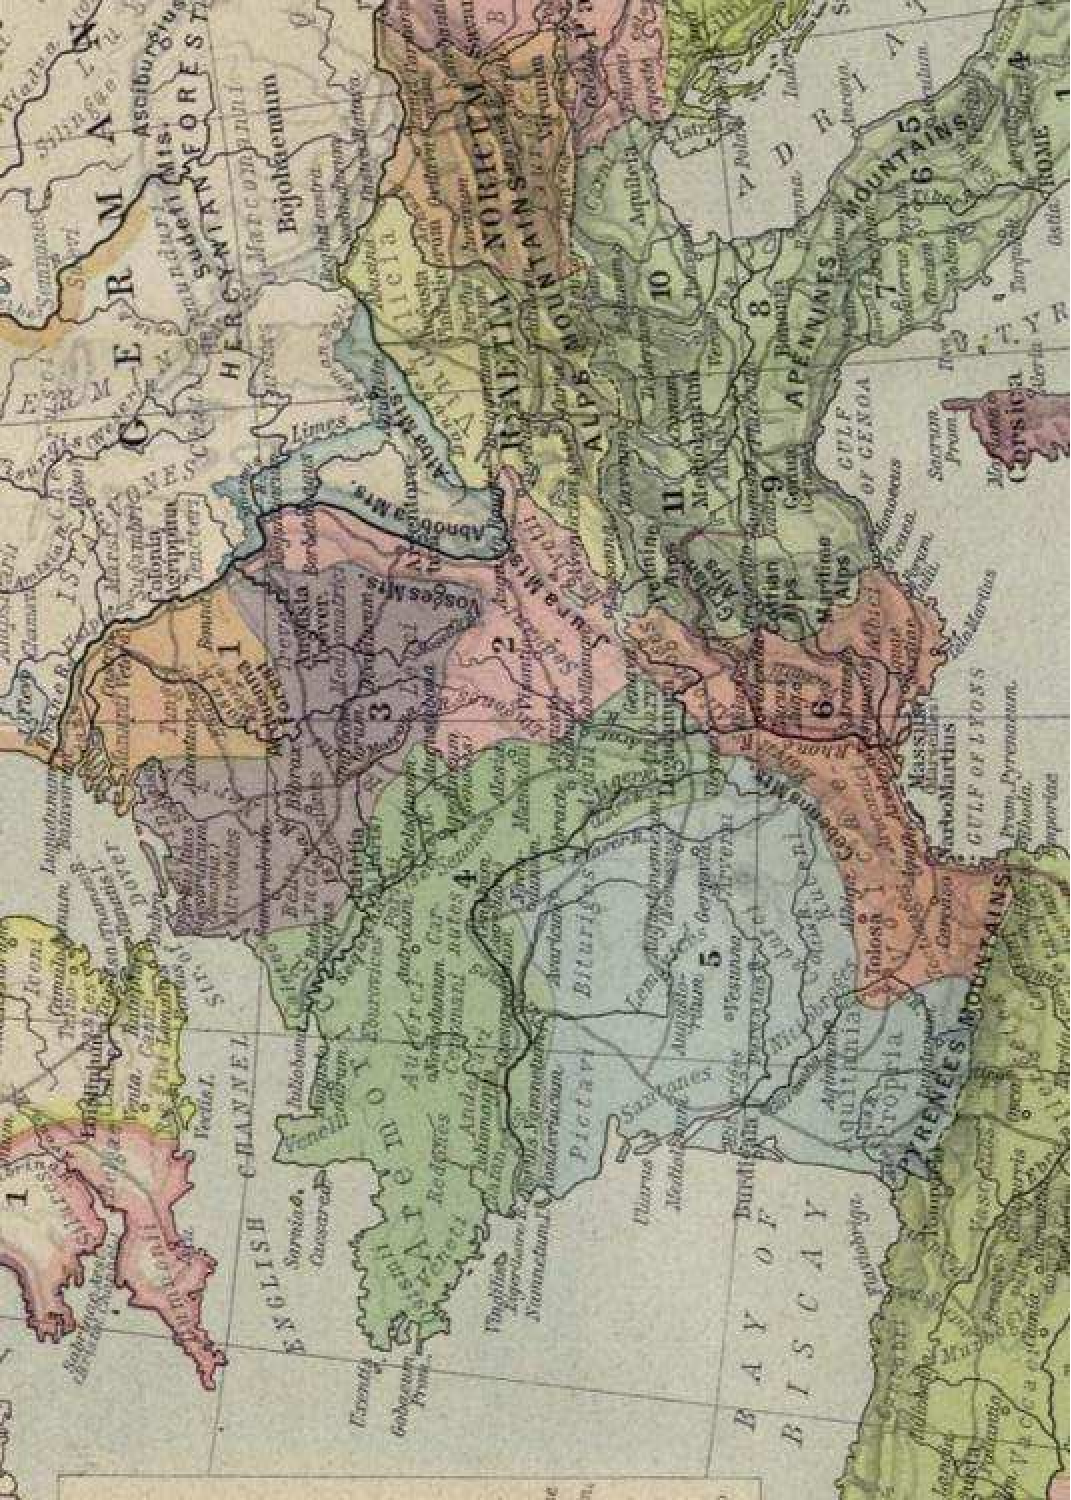
\includegraphics[width=175pt, angle=270]{bilder/Galia}
  \caption{Gallien zur Zeit Caesars}\label{fig_Gallien}
\end{center}
\end{figure}


\begin{table}[htb]
\begin{center}
\begin{tabular}{|l|l|l|}
\hline
Jahr &  Erster Consul & Zweiter Consul\\
\hline \hline
1 & C. Caesar         & L. Aemilius Paullus\\
2 & P. Vinicius       & P. Alfenus Varus\\
3 & L. Aelius Lamia   & M. Servilius\\
4 & Sex. Aelius Catus &  C. Sentius Saturninus\\
5 & L. Valerius Messalla& Cn. Cornelius Cinna \\
suff. & C. Vibius Postumus &  C. Ateius Capito\\
6 & M. Aemilius Lepidus & L. Arruntius\\
\hline
\end{tabular}
 \caption{Römische Konsulen}\label{tab_Konsulen}
\end{center}
\end{table}


\pagebreak

\section{De Bello Hispaniensi}\raggedbottom 

Pharnace superato, Africa recepta, qui ex his proeliis cum
adulescente Cn. 

\pagebreak
\section{Weiteres Kapitel}\raggedbottom 
\subsection{Unterkapitel}
\subsection{Unterkapitel}


\section{Alte Version} \raggedbottom 

Der Haupthistokompatibilitätskomplex, kurz MHC, ist ein Teilstück der DNA von Wirbeltieren, welches unter anderem eine tragende Rolle bei Vorgängen des Immunsystems besitzt. Somit besteht besonders großes Forschungsinteresse an der Untersuchung dieses Abschnittes. Daten über dieses Teilstück liegen jedoch nur, wie generell bei DNA üblich, fragmentweise vor. Diese Fragmente werden auch Contigs genannt. Somit bildet das Zusammenfügen bzw. Assemblieren der einzelnen Contigs eine Herausforderung, um weiterer Forschung den Weg zu bereiten. 

Diese Arbeit entsteht in Zusammenarbeit mit der Manchot-Forschungsgruppe vom Institut für Medizinische Mikrobiologie und Krankenhaushygiene der HHU, welche Daten zur APD, einer bestimmten Zelllinie des menschlichen Hauptkompatibilitätskomplex, zur Verfügung gestellt haben. 
%Für die Bearbeitung dieser Abschlussarbeit liegen Daten zur APD, einer bestimmten Zelllinie des menschlichen Hauptkompatibilitätskomplex, vor. 
Die Daten bestehen aus gemessenen Distanzen von je zwei Contigs, sogenannten Constraints. 
Das Ziel ist es, mithilfe von Methoden der linearen Programmierung, eine Rekonstruktion des Teilstücks der DNA vorzunehmen. Faktoren, die dieses Zusammenfügen erschweren, sind zum einen Mehrfachauflistungen gleicher Contigs-Paare mit schwankenden Distanzen. Zum anderen können auch widersprüchliche Distanzen auftreten, zum Beispiel können Teile der Daten eine Kreisbildung suggerieren, welche so in einem Chromosom nicht auftreten kann. Eine mögliche Erklärung dafür ist ein Mehrfachauftreten eines Contigs - auch genannt Repeat. Letztlich bleibt noch die große Datenfülle als Herausforderung zu nennen: Bei rund 122\,000 auftretenden Distanzen zwischen 2\,124 Contigs ist eine manuelle Zusammenfügung nicht zielführend und mindestens eine Teilautomatisierung der Prozesse obligatorisch.

Die Arbeit ist wie folgt aufgebaut:\\


...